\documentclass[12pt]{article}
\usepackage{graphicx}
\usepackage{amsmath}
%
\begin{document}
\title{Constructing Composite Stellar Profiles}
\author{Robert Lupton}
%\date{Today}
\maketitle

\section{Introduction}

If you have a set of profiles for number of stars, with each profile
covering the same range of radii, deriving a composite profile is
simple; simply add together all the profiles,
without any clever weights (i.e. add together all the
photons from all the stars). If some of the stars have missing points
on their profiles, as is the case if some are saturated, things are
not so straightforward, but a simple procedure is derived in the next
section.

In determining stellar power-law wings such a procedure is required; you
need to know the PSF's core shape (and magnitude), while only for
saturated stars is the wing shape well determined, and reasonably insensitive
to the sky level.

\section{Theory}

Let us assume that we have a set of $N$ radial profiles of stars, each
of which has $n$ points; write the $i^{th}$ point on the $j^{th}$ profile
as $P_i^j$. If all the profiles are identical except for a scale
factor $\alpha^j$, we have
$$
P_i^j = \alpha^j f_i + \epsilon_{ij}
$$
with $\langle{\epsilon_{ij}}\rangle = 0$ and
$\langle{\epsilon_{ij}^2}\rangle = \sigma_{ij}^2$; we assume that the
$\epsilon_{ij}$ for different $i$ and $j$ are independent.

Taking a logarithm on each side, this becomes
\footnote{We have of course introduced a small bias by this procedure.
If $x$ has mean $\langle{x}\rangle \equiv \mu$ and variance $\sigma^2$, then
$\langle{\ln{x}}\rangle \approx \ln\mu - \sigma^2/(2\mu^2)$}
\begin{align*}
\ln P_i^j &= \ln\alpha^j + \ln f_i +
		\ln\left(1 + \frac{\epsilon_{ij}}{\alpha^j f_i}\right)\\
          &\sim \ln\alpha^j + \ln f_i +
		\frac{\epsilon_{ij}}{\alpha^j f_i}
\end{align*}
If we write the error term as $\epsilon_{ij}/P_i^j$ this is a
linear problem, which can be written in canonical form
${\bf y} = M \mbox{\boldmath $\theta$} + \mbox{\boldmath $\epsilon$}$,
where ${\bf y}$ represents the vector of the $P_i^j$s,
$M$ a matrix of coefficients,
{\boldmath $\theta$} a vector of $\ln\alpha$ and $\ln f$,
and {\boldmath $\epsilon$} a vector of errors. Specifically,
\begin{eqnarray*}
\left(\begin{array}{c}
	\ln P_1^1\\ \ln P_2^1\\ \vdots\\ \ln P_1^2\\ \ln P_2^2\\ \vdots \\ \ln P_{n-1}^N\\ \ln P_n^N
\end{array}\right)
=
\left(\begin{array}{cccc|cccc}
	1 & 0 & \ldots & 0 & 1 & 0 & \ldots & 0 \\
	0 & 1 & \ldots & 0 & 1 & 0 & \ldots & 0 \\
	\vdots& \vdots& \ddots& \vdots& \vdots& \vdots& \ddots& \vdots\\
\hline
	1 & 0 & \ldots & 0 & 0 & 1 & \ldots & 0 \\
	0 & 1 & \ldots & 0 & 0 & 1 & \ldots & 0 \\
	\vdots& \vdots& \ddots& \vdots& \vdots& \vdots& \ddots& \vdots\\
\hline
	\vdots& \vdots& \ddots& \vdots& \vdots& \vdots& \ddots& \vdots\\
	0 & 0 & \ldots & 1 & 0 & 0 & \ldots & 1 \\
\end{array}\right)
\left(\begin{array}{c}
	\ln f_1 \\ \ln f_2 \\ \vdots \\ \ln f_n \\
	\hline
	\ln\alpha_1 \\ \ln\alpha_2 \\ \vdots \\ \ln\alpha_N
\end{array}\right)
+ 
\left(\begin{array}{c}
	\epsilon_{11}/P_1^1\\
	\epsilon_{21}/P_2^1\\
	\vdots\\
	\epsilon_{12}/P_1^2\\
	\epsilon_{22}/P_2^2\\
	\vdots\\
	\epsilon_{n-1,N}/P_{n-1}^N\\
	\epsilon_{nN}/P_n^N
\end{array}\right)
\end{eqnarray*}

Let us write $W_{ij} \equiv \left(P_i^j/\sigma_{ij}\right)^2$, so that
{\boldmath $\epsilon$}'s covariance matrix $V$ is simply
\begin{eqnarray*}
V = \left(\begin{array}{cccc}
	1/W_{11} & 0 & 0 & \ldots \\
	0 & 1/W_{21} & 0 & \ldots \\
	0 & 0 & 1/W_{31} & \ldots \\
	\vdots & \vdots & \vdots& \ddots \\
\end{array}\right)
\end{eqnarray*}

The minimum-least-squares estimate for the $\ln f_i$ and $\ln\alpha^j$
is given by $\left(M^T V^{-1}\! M\right)^{-1} M^T V^{-1} {\bf y} = $
\begin{eqnarray*}
\left(\begin{array}{cccc|ccccc}
	\sum_j W_{1j} & 0 & \ldots & 0 &
			W_{11} & W_{12} & \ldots & W_{1N} \\
	0 & \sum_j W_{2j} & \ldots & 0 &
			W_{21} & W_{22} & \ldots & W_{2N} \\
	\vdots &\vdots& \ddots  & \vdots  & \vdots & \vdots & \ddots & \vdots\\
	0 & 0 & \ldots & \sum_j W_{nj} &
			W_{n1} & W_{n2} & \ldots & W_{nN} \\
\hline
	W_{11} & W_{21} & \ldots & W_{n1} &
			\sum_i W_{i1} & 0 & \ldots & 0 \\
	W_{12} & W_{22} & \ldots & W_{n2} &
			0 & \sum_i W_{i2} & \ldots & 0 \\
	\vdots &\vdots& \ddots  & \vdots  & \vdots & \vdots &\ddots & \vdots\\
	W_{1N} & W_{2N} & \ldots & W_{nN} &
			0 & 0 & \ldots & \sum_i W_{iN} \\
\end{array}\right)^{-1}
\left(\begin{array}{c}
\sum_j W_{1j} \ln P_1^j \\
\sum_j W_{2j} \ln P_2^j \\
\vdots \\
\sum_j W_{nj} \ln P_n^j \\
\hline
\sum_i W_{i1} \ln P_i^1 \\
\sum_i W_{i2} \ln P_i^2 \\
\vdots \\
\sum_i W_{iN} \ln P_i^N \\
\end{array}\right)
\end{eqnarray*}

%%For the case that all of the $W_{ij}$ are equal, this becomes
%%\begin{eqnarray*}
%%\left(\begin{array}{cccc|ccccc}
%%	N & 0 & \ldots & 0 & 1 & 1 & \ldots & 1 \\
%%	0 & N & \ldots & 0 & 1 & 1 & \ldots & 1 \\
%%	\vdots &\vdots& \ddots  & \vdots  & \vdots & \vdots & \ddots & \vdots\\
%%	0 & 0 & \ldots & N & 1 & 1 & \ldots & 1 \\
%%\hline
%%	1 & 1 & \ldots & 1 & n & 0 & \ldots & 0 \\
%%	1 & 1 & \ldots & 1 & 0 & n & \ldots & 0 \\
%%	\vdots &\vdots& \ddots  & \vdots  & \vdots & \vdots &\ddots & \vdots\\
%%	1 & 1 & \ldots & 1 & 0 & 0 & \ldots & n \\
%%\end{array}\right)^{-1}
%%\left(\begin{array}{c}
%%\sum_j \ln P_1^j \\
%%\sum_j \ln P_2^j \\
%%\vdots \\
%%\sum_j \ln P_n^j \\
%%\hline
%%\sum_i \ln P_i^1 \\
%%\sum_i \ln P_i^2 \\
%%\vdots \\
%%\sum_i \ln P_i^N \\
%%\end{array}\right)
%%\end{eqnarray*}

This matrix is singular, as one of the $\alpha^j$s simply sets the scale
for the composite profile $f_i$; I have chosen to solve this problem by
setting $f_1 = 1$ and deleting the first row of $M$ and consequently the first row and column from
$M^T V^{-1}\! M$ (equivalently, you could set $\alpha_0 = 1$ and eliminate {\em its} row
and column --- but this would mean that all the uncertainty in scaling the
first profile to the composite appears in the composite's error bars).

If a point in the profile is missing, you can simply set the corresponding
$W_{ij}$ to zero; providing that each pair of neighbouring points is
represented in at least one of the input profiles, and that each profile
contains at least two usable points, the matrix should not be singular.

The covariance matrix for the $\ln f_i$ and $\ln\alpha^j$ is given by
$\left(M^T V^{-1}\! M\right)^{-1}$

\section{Example from Photo}

A simulated $r'$ frame was run through photo's correct frames and bright
object finder, resulting in a list of 11 objects with more than 100000 counts,
or about 16th magnitude. Their profiles are shown in the figure, along
with the derived composite profile. Note that this composite is {\em not}
a Gaussian-plus-powerlaw fit to the data, it is simply the $f_i$ derived
as in the previous section, scaled by the $\alpha^j$.

\begin{figure}
\begin{center}
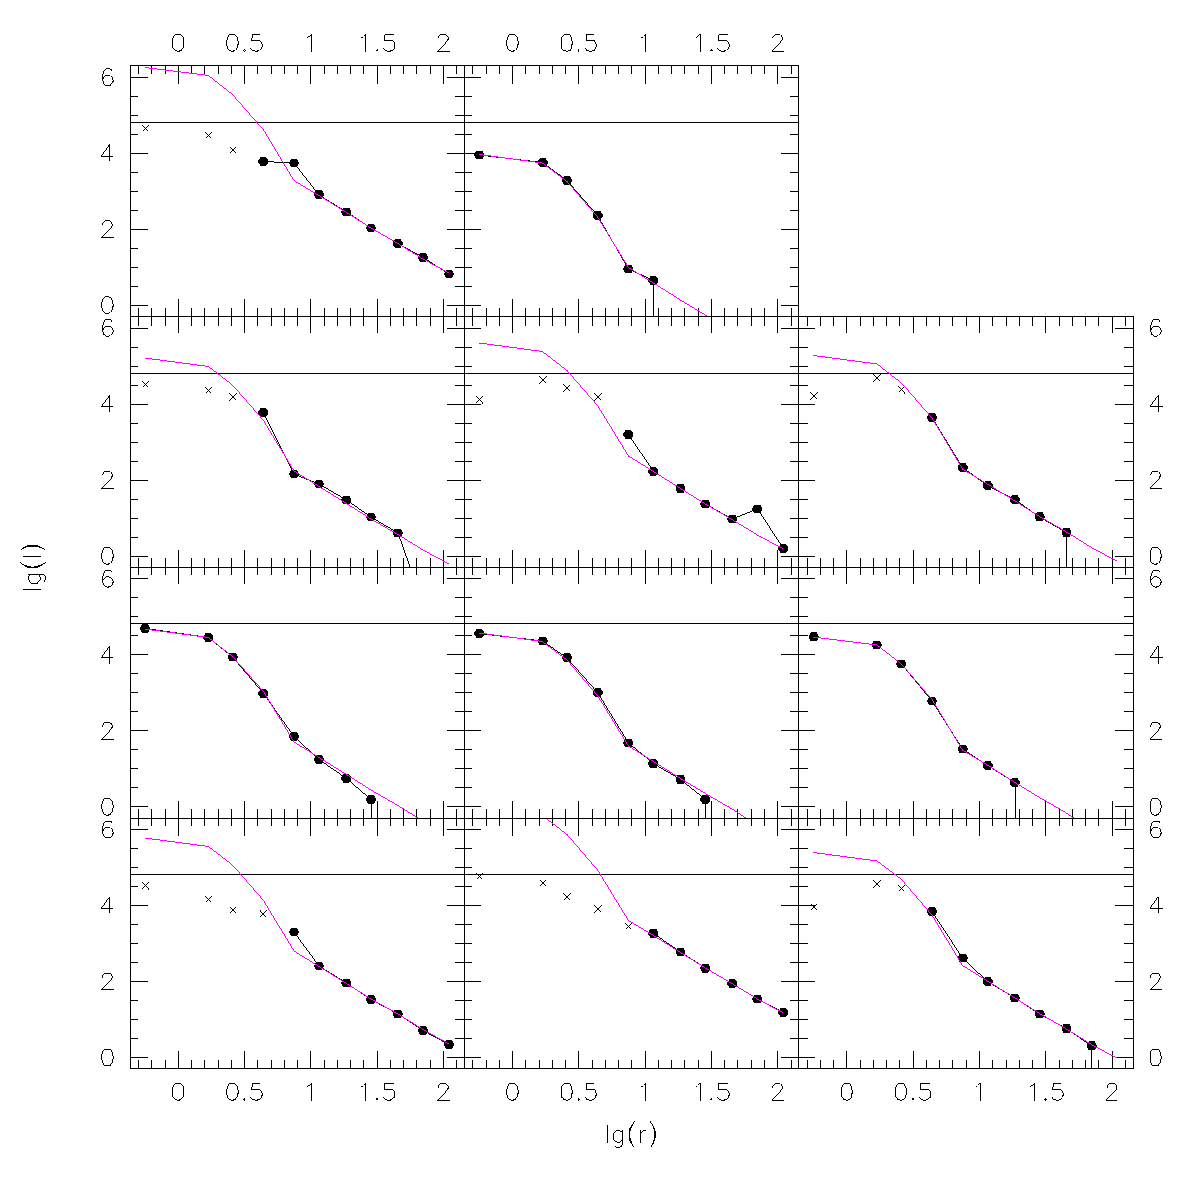
\includegraphics[width=6in]{composite_star}
\end{center}
% \centerline{\epsfxsize=6in \epsfbox{composite_star.ps}}
\caption{The radial profiles of 11 stars from a simulated photo frame.
For each star, the solid points are those used to derive the composite,
while the crosses mark points that may have been contaminated by saturation.
The magenta line indicates the derived composite profile scaled to the
data; the horizontal black line is the saturation level of the chip.
}
\end{figure}


\end{document}
